\documentclass[tikz,border=10pt]{standalone}
\usepackage{tikz}
\usetikzlibrary{trees,arrows.meta,positioning,calc}

\begin{document}
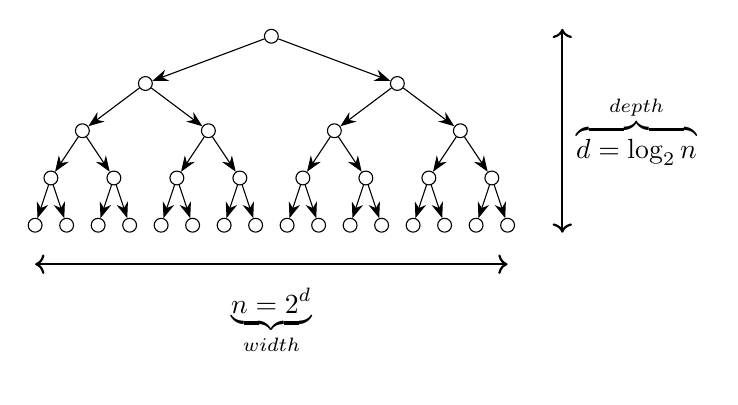
\begin{tikzpicture}[
  level distance=6mm,
  level 1/.style={sibling distance=32mm},
  level 2/.style={sibling distance=16mm},
  level 3/.style={sibling distance=8mm},
  level 4/.style={sibling distance=4mm},
  every node/.style={circle,draw,inner sep=1pt,minimum size=5pt},
  edge from parent/.style={draw,-{Stealth[length=2mm]}}
]

% ---------- binary tree with 16 leaves ----------
\node (root) {}
 child { node {}
   child { node {}
     child { node {}
       child { node (L) {} } child { node {} }
     }
     child { node {}
       child { node {} } child { node {} }
     }
   }
   child { node {}
     child { node {}
       child { node {} } child { node {} }
     }
     child { node {}
       child { node {} } child { node {} }
     }
   }
 }
 child { node {}
   child { node {}
     child { node {}
       child { node {} } child { node {} }
     }
     child { node {}
       child { node {} } child { node {} }
     }
   }
   child { node {}
     child { node {}
       child { node {} } child { node {} }
     }
     child { node {}
       child { node {} } child { node (R) {} }
     }
   }
 };

% ---------- vertical height arrow ----------
\coordinate (rightside) at ($(R.east)+(6mm,0)$);
\draw[<->,thick]
  (rightside |- root.north) --
  node[right,midway,draw=none] {$\overbrace{d = \log_2 n}^{\text depth}$}
  (rightside |- R.south);

% ---------- horizontal width arrow ----------
\coordinate (Lbot) at ($(L.south)-(0,4mm)$);
\coordinate (Rbot) at ($(R.south)-(0,4mm)$);
\draw[<->,thick] (Lbot) -- node[below,draw=none] {$\underbrace{n = 2^d}_{\text{width}}$} (Rbot);

\end{tikzpicture}
\end{document}
